
\textbf{Komponenten\hyperlink{LF01_Link}{/LF01/}} \\

\begin{wrapfigure}{r}{0.4\textwidth} % Increase the width of the figure environment
	\vspace{-60pt + 0.02\textwidth}
	\hspace{0.07\textwidth} % Add horizontal space
	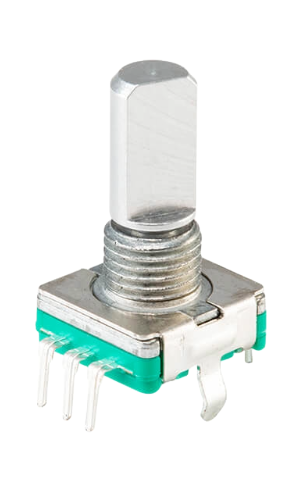
\includegraphics[width=0.2\textwidth]{images/05_technische_spezifikation/Interface/Encoder.png} % Keep the image size the same
	\caption{Rotary-Encoder}
	\label{fig:rotary_encoder}
	\vspace{-100pt}
\end{wrapfigure}

\textbf{\hypertarget{Encoder}{Encoder}} \\

\textbf{Model} RIC11-22S16D5M-TH

\textbf{Spannung} 3.3V

\textbf{Mechanisch:}
\begin{itemize}
	\item 20 Impulse pro Umdrehung (20 PPR)
	\item 20 Positionen (20 DET)
	\item Schalter (SW)
\end{itemize} 



Zur Auswahl der Samples und zum Navigieren durch das Menü wir ein Rotary-Encoder mit einem Switch Button eingesetzt.Das Empfangen der \textbf{A} und \textbf{B} Signale des Encoders erfolgt über die Pins \boldinline{PA0} und \boldinline{PA1}.
Das Drücken des Switch über den Pin \boldinline{PA4}. Durch das drücken des Switch-Buttons wird der Pin \boldinline{PA4} auf high gesetzt.

\begin{itemize}
	\item \textbf{Präzise Steuerung:} Der Encoder ermöglicht eine präzise Steuerung des Cursors auf dem Display.
	
	\item \textbf{Benutzerfreundlichkeit:} Der Benutzer kann durch die Liste navigieren und ein Sample auswählen. Die Kombination aus Drehbewegung und Druckknopf-Funktionalität macht den Encoder intuitiv.  
\end{itemize}

\vspace{3em}

\begin{wrapfigure}{r}{0.4\textwidth} % Increase the width of the figure environment
	\vspace{-20pt + 0.02\textwidth}
	\hspace{0.06\textwidth} % Add horizontal space
	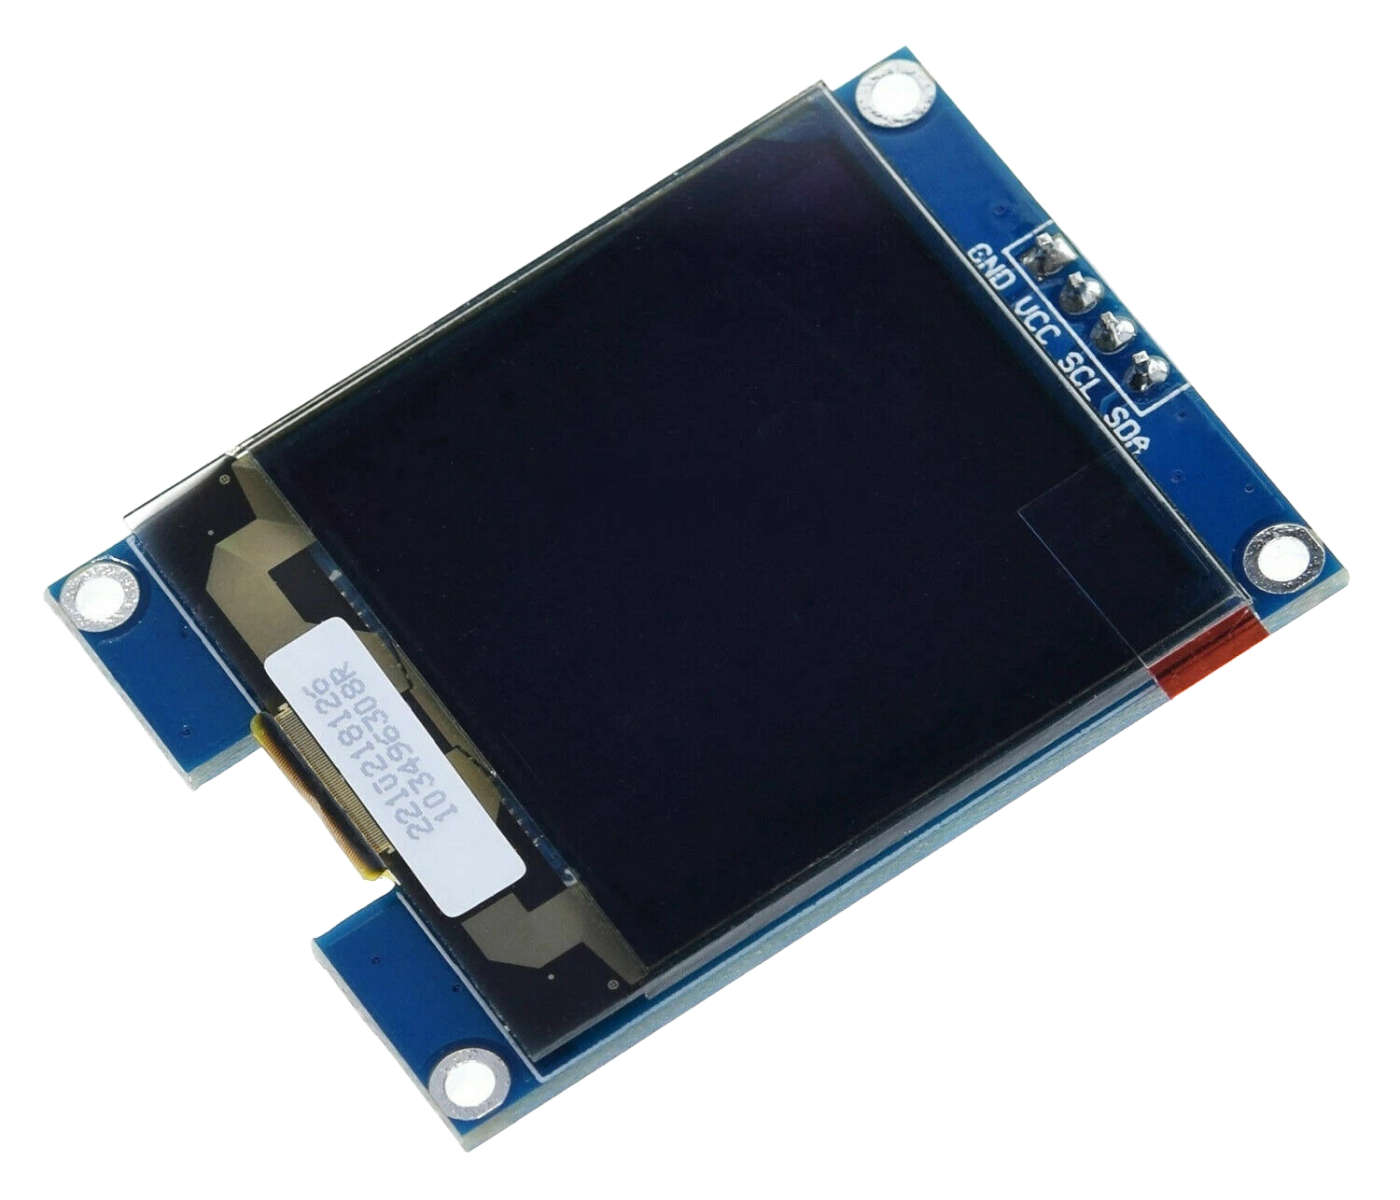
\includegraphics[width=0.25\textwidth]{images/05_technische_spezifikation/Interface/Display.png} % Keep the image size the same
	\caption{LCD-Display}
	\label{fig:lcd_display}
	\vspace{-50pt}
\end{wrapfigure}

\textbf{\hypertarget{Display}{LCD-Display}} \\

\textbf{Model:} GME128128-01-ii2

\textbf{Treiber:} SH1107

\textbf{Mode} Monochrom (1Bit)

\textbf{Spannung} 5.0V \\ \\



Zur Visualiesierung der Sampels haben wir einen Monochronen LCD-Display benutzt. Im zusammenspiel mit dem Encoder ermöglicht es eine gute Navigation durch den gewünschten Samplepool. Die Daten werden über den Output Pin  \boldinline{PB7} an den SDA des Displays übertragen. Der Takt wird über den Pin  \boldinline{PB6} an den SCL übertragen. Das Display wird mit 20 FPS betrieben und mit hilfe von \boldinline{Timer tim5} geupdated.

\begin{itemize}
	\item \textbf{Klare Visualisierung:} LCD-Displays bieten eine klare und gut lesbare Darstellung von Text und Grafiken.
	\item \textbf{Anpassbarkeit:} Sie können einfach an verschiedene Layouts und Designs angepasst werden.
\end{itemize}

\newpage
\textbf{Komponenten\hyperlink{LF02_Link}{/LF02/}} \\

\textbf{\hypertarget{Potentiometer}{Schiebe-Potentiometer}}\\

\textbf{Model} Bourns PTL45-15R0-103B2

\textbf{Wiederstand} 10k Ohm

\textbf{Weg} 100mm

\textbf{Spannung} 3.3V \\ \\ \\

	\begin{wrapfigure}{r}{0.4\textwidth} % Increase the width of the figure environment
	\vspace{-155pt + 0.02\textwidth}
	\hspace{0.07\textwidth} % Add horizontal space
	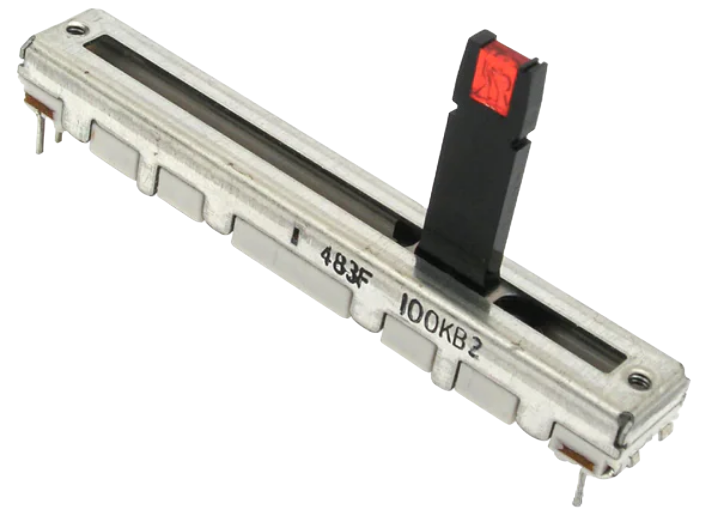
\includegraphics[width=0.2\textwidth]{images/05_technische_spezifikation/Interface/Potentiometer.png} % Keep the image size the same
	\caption{Potentiometer}
	\label{fig:schiebe_potentiometer}
	\vspace{-20pt}
\end{wrapfigure}

Für die Filterfunktion benötigen wir 5 Potentiometer. Es wird zyklisch die Ausgangsspannung des Schleifers abgegriffen die die Teilspannung zwichen den VCC und dem GND darstellt. Dies erfolgt mit Hilfe vom ADC und dem DMA. Die Auswertung der Spannung erfolgt über die Pins  \boldinline{PA6, PA7, PB0, PB1, PC0}. Die Pins  \boldinline{PA6, PA7, PB0, PB1} sind für die Klassen zuständig  \boldinline{PC0} für den Schwellenwert an erlaubter Abweichung.

\begin{itemize}
	\item \textbf{Präzise Steuerung und feine Abstimmung:} Ein Potentiometer ermöglicht eine stufenlose und präzise Einstellung. Durch das Schieben des Potentiometers kann der Benutzer den Cursor in kleinen, genauen Schritten bewegen.
	\item \textbf{Einfache Bedienung und intuitive Nutzung:} Potentiometer sind einfach und intuitiv zu bedienen.
	\item \textbf{Direkte visuelle Rückmeldung:} Durch die sofortige visuelle Rückmeldung auf dem LCD-Display kann der Benutzer sofort sehen, wie sich die Bewegung des Potentiometers auf die Position des Cursors auswirkt.
\end{itemize}


\textbf{(LCD-Display)}\\

Der LCD-Display ist der gleiche wie im \boldinline{/LF01/} beschrieben. Dieser dient zur Darstellung der Fader Einstellung in prozentualer Form.

\newpage

\subsubsection{Pinout Interface Komponente}

\textbf{Interface}

\begin{longtable}[c]{|p{2.5cm}|p{1cm}|p{2.5cm}|p{2.5cm}|p{2.5cm}|p{3cm}|}
	\hline
	\textbf{Komponente} & \textbf{PIN} & \textbf{Signal-On-PIN} &  \textbf{GPIO-Mode} & \textbf{GPIO-Pull-Up/Pull-Down } & \textbf{User-Label}\\
	\hline
	Encoder Menü & PA0 & n/a & EIMRETD & PULL UP & enc\_a\_clk\_in1 \\
	\hline
	& PA1 & n/a &  INPUT & PULL UP & enc\_a\_dt\_in2 \\
	\hline
	& PA4 & n/a & EIMRETD & PULL UP & enc\_a\_switch\_in3 \\
	\hline
	ADC & PA6 & ADC1\_IN6 & ANALOG & NPU NPD & FADER1 \\
	\hline
	& PA7 & ADC1\_IN7 & ANALOG & NPU NPD & FADER2 \\
	\hline
	& PB0 & ADC1\_IN8 & ANALOG & NPU NPD & FADER3 \\
	\hline
	& PB1 & ADC1\_IN9 & ANALOG & NPU NPD & FADER4 \\
	\hline
	& PC0 & ADC1\_IN10 & ANALOG & NPU NPD & FADER5 \\	
	\hline
	I2C & PB6 &I2C1\_SCL & AFOD & PULL UP & n/a \\
	\hline
	& PB7 &I2C1\_SDA & AFOD & PULL UP & n/a \\
	\hline
	SDIO & PC8 & SDIO\_D0 & AFPP & PULL UP & n/a \\
	\hline
	& PC9 & SDIO\_D1 & AFPP & PULL UP & n/a \\
	\hline
	& PC10 & SDIO\_D2 & AFPP & PULL UP & n/a \\
	\hline
	& PC11 & SDIO\_D3 & AFPP & PULL UP & n/a \\
	\hline
	& PC12 & SDIO\_CK & AFPP & NPU NPD & n/a \\
	\hline
	& PD2 & SDIO\_CMD & AFPP & PULL UP & n/a \\
	\hline
\end{longtable}

\textbf{EIMRETD} = External Interrupt Mode and Rising Edge Trigger Detection 		

\textbf{AFOD} = Alternate Function Open Drain

\textbf{NPU NPD} = No Pull Up No Pull Down		

\textbf{AFPP} = Alternate Function Push Pull

